\chapter*{ ANTON-BIVENS-DAVIS 3.1 EJERCICIO 40}

\textbf{39-40:} Se dice que dos curvas son \textbf{ortogonales} si sus líneas tangentes son perpendiculares en cada punto de intersección, y dos familias de curvas son \textbf{trayectorias ortogonales} una de otra, si cada miembro de la familia, es ortogonal de otro miembro de la otra familia. Esta terminología es usada en estos ejercicios. \newline

\textbf{40.} La figura muestra algunos miembros típicos de la familia de hiperbolas $xy = c$ (curvas negras) y $x^{2} - y^{2} = k$ (curvas grises), donde $ c \neq 0$ y $ k \neq 0$. Usar la pista de 39 para mostrar que estas familias son trayectorias ortogonales una de otra. [*HINT 39: Para que las rectas tangentes sean perpendiculares en un punto de la intersección, las pendientes de esas rectas tangentes deber ser recíprocas negativas una de otra]. \\
\newline
\begin{center}
    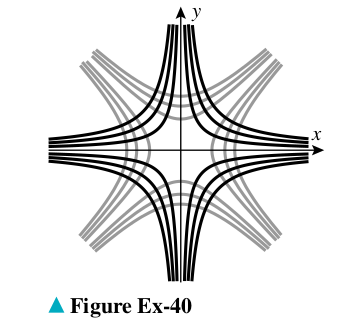
\includegraphics[height = 0.25\textheight]{recursos/Grafo40.png}\par
\end{center}

\textbf{Desarrollo:}\newline
Se debe mostrar que para cada miembro de la familia $xy = c$ hay una curva ortogonal a ella en la familia  $x^{2} - y^{2} = k$ . \\
Para esto las pendientes de estas dos curvas deber ser el recíproco negativo de la otra pendiente. (La pendiente de la recta tangente en un punto es la derivada).\\
\newline
\textbf{1) Derivar:} Derivar las ecuaciones de cada familia, tomando a $c$ y $k$ como constantes. (Derivación implícita).
\begin{align*}
   xy &= c           &... (1)\\
   x^{2} - y^{2} &= k              &...(2)
\end{align*}
\newline
\textbf{Derivando (1):}
\begin{align*}
    \frac{d}{dx}xy &= \frac{d}{dx}c \\
    \frac{d}{dx}xy &= 0 \\
    x\frac{d}{dx}y  +  y\frac{d}{dx}x &= 0 \\
    x\frac{dy}{dx} +  y(1) &= 0 \\
    x\frac{dy}{dx}  &= -y \\
    \frac{dy}{dx}  &= -\frac{y}{x}\\
    m_{1}  &= -\frac{y}{x}
\end{align*}
\newline
\textbf{Derivando (2):}
\begin{align*}
    \frac{d}{dx}(x^{2} - y^{2}) &= \frac{d}{dx}k \\
    \frac{d}{dx}x^{2} -  \frac{d}{dx}y^{2} &= 0\\
    2x -  2y\frac{d}{dx}y &= 0\\
    -2y\frac{dy}{dx} &= -2x\\
    \frac{dy}{dx} &= \frac{-2x}{-2y}\\
    \frac{dy}{dx} &= \frac{x}{y}\\
    m_{2}  &= \frac{x}{y}
\end{align*}
\newline
\textbf{Ahora} teniendo ambas pendientes, el recíproco negativo de una debe ser la otra. \\
\begin{center}
    $ m_{1}  = -\frac{1}{m_{2}}$      y    $ m_{2}  = -\frac{1}{m_{1}}$\\
\end{center}
\textbf{Entonces:}
\begin{center}
    Si $ m_{1}  = -\frac{y}{x} $ \\
    $\Rightarrow$ 
\end{center}
\begin{align*}
   -\frac{1}{m_{1}} &= -\frac{1}{-\frac{y}{x}}\\
   -\frac{1}{m_{1}} &= -\frac{\frac{1}{1}}{-\frac{y}{x}}\\
   -\frac{1}{m_{1}} &= -\frac{1(x)}{1(-y)}\\
   -\frac{1}{m_{1}} &= -\frac{x}{-y}\\
   -\frac{1}{m_{1}} &= \frac{x}{y}\\
\end{align*}
\[
  -\frac{1}{m_{1}} = \frac{x}{y} = m_{2}
\]
\[
\therefore  m_{1}  = -\frac{1}{m_{2}}   \Leftrightarrow   m_{2}  = -\frac{1}{m_{1}}
\]
\newline
Ambas pendientes son la recíproca negativa de la otra. Así podemos decir que estas familias de curvas son trayectorias ortogonales.